\chapter{Diffusion measurements in the CERN LHC}

\section{The LHC collimator system}

%%%%%%%%%%%%%%%%%%%%%%%%%%%%%%%%%%%% IPAC 2022 %%%%%%%%%%%%%%%%%%%%%%%%%%%%%%%%%%%%

In high-energy colliders or storage rings bound to use superconducting magnets, the beam dynamics is extremely complex and intrinsically nonlinear, due to the unavoidable magnetic field errors. This might generate beam losses or emittance growth that affect the accelerator performance, either because of a reduction of the luminosity or due to a reduction of the operational efficiency. A link between dynamic aperture (DA), i.e. the extent of the phase-space region in which bounded motion occurs, and beam lifetime has been established~\cite{PhysRevSTAB.15.024001} and successfully used to measure DA~\cite{PhysRevAccelBeams.22.034002}. However, this approach does not give any hint on the evolution of the beam distribution, which provides means to predict the beam losses and lifetime, and, more importantly, also the evolution of the beam emittance. This is crucial to assess the presence of emittance growth phenomena, which play a role in determining the actual performance of the collider or storage ring. 

In this respect, the development of a framework based on diffusive models of the non-linear beam dynamics is particularly useful. The approach followed is to construct a Fokker-Planck (FP) equation that gives access to the evolution of the beam distribution over time scales compatible with those of physical interest (direct tracking of $10^8$ turns for several initial conditions for a complex lattice like the LHC one is still not an option nowadays). The development of diffusive models of the transverse beam dynamics is not new for accelerator physics (see, e.g.~\cite{PhysRevLett.68.33,gerasimov1992applicability,MESS1994279,zimmermann1994transverse,PhysRevLett.77.1051,PhysRevSTAB.5.074001,stancari2011diffusion,PhysRevSTAB.15.101001} and references therein). However, recently a new framework has been developed~\cite{Bazzani:2019lse,bazzani2020diffusion,our_paper9}, in which the functional form of the diffusion coefficient is derived from the optimal estimate of the perturbation series provided by the Nekhoroshev theorem~\cite{Nekhoroshev:1977aa,Bazzani:1990aa,Turchetti:1990aa}. 
The FP equation describes the time evolution of the beam distribution $\rho$ according to 
%
\begin{equation}
    \begin{split}
        \frac{\partial \rho (I, t)}{\partial t} & =\frac{1}{2} \frac{\partial}{\partial I} {D}(I) \frac{\partial}{\partial I}\, \rho(I, t) \\
        D(I) & \propto\exp \left[-2\left({I_\ast} / {I}\right)^{\frac{1}{2\kappa}}\right]\, , 
    \end{split}
    \label{eq:fp}
\end{equation}
%
where $D(I)$ is the diffusion coefficient as a function of the action variable $I$. % has been used. 
Equation~(\ref{eq:fp}) is suitable for studying the evolution of beam distributions in the presence of collimators with jaws that provide %can be represented by 
absorbing boundary conditions necessary to solve the FP equation. Note that the so-called collimator scans, i.e. the controlled movement of the jaws of the LHC collimators, can be used to study beam-halo dynamics and, in particular, to reconstruct the diffusion coefficient behaviour as a function of transverse amplitude~\cite{MESS1994279,stancari2011diffusion,PhysRevSTAB.16.021003,PhysRevAccelBeams.23.044802}. The collimator scan method is widely used in LHC operation and is based on small jaw displacements at different amplitudes $I$, combined with measurement of beam losses. Displacements can be inward or outward, causing different characteristic profiles of beam losses. 

The special functional form of the diffusion coefficient is related to the functional form provided by the estimate of the optimal perturbation series, according to the Nekhoroshev theorem~\cite{Turchetti:1990aa,Bazzani:1990aa}. The parameters $\kappa, I_\ast$ have a physical meaning that stems from the Nekhoroshev theorem: the exponent $\kappa$ is related to the analytic structure of the perturbative series and to the dimensionality of the system~\cite{bazzani2020diffusion}; $I_\ast$ is related to the asymptotic character of the perturbative series.
%
\section{Probing $D(I)$ from loss data}
%
\begin{figure*}[t]
    \centering
    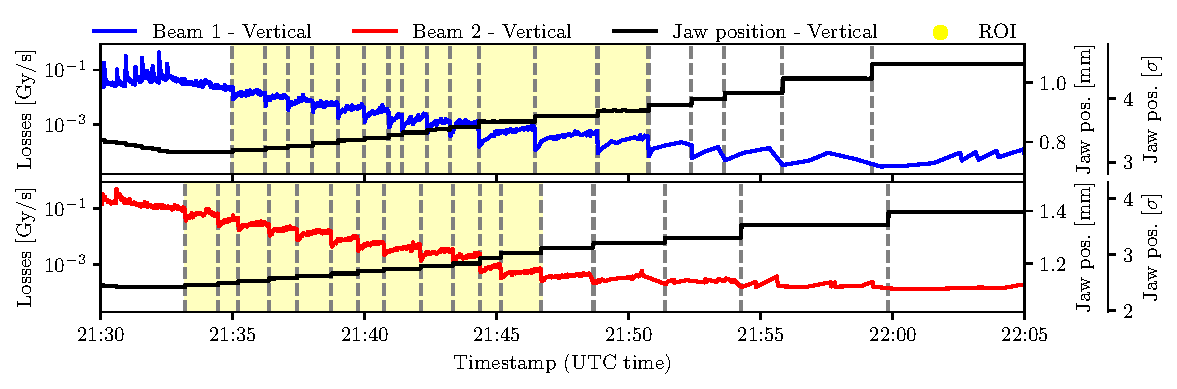
\includegraphics[trim={0 2.5mm 0 4mm}, clip, width=\textwidth]{5_Diffusion_measurement_LHC/figs/first.pdf}
    \caption{Beam losses from the BLM monitor (i.e.\ the maximum spike over a time window of \SI{10.24}{ms}) and jaw positions measured in the vertical plane for the collimator scans carried out in fill 6052. The data shown correspond to outward jaw movements. The yellow-marked region of interest (ROI) represents a subset of data meeting our quality requirements~\cite{PhysRevAccelBeams.23.044802}.}
    \label{fig:first}
\end{figure*}

A recent work~\cite{our_paper9}, considered a measurement protocol for probing a Nekhoroshev-like diffusive behaviour of the beam halo. It is based on alternating inward and outward jaw movements during collimator scan measurements. The idea behind the proposed protocol is that the observed current loss signal $J(t)$ can be divided into two separate processes with different timescales: (1) a global process $J_\text{eq}(t)$ generated by exponentially slow erosion of the beam core and (2) a recovery current $J_\mathrm{R}(t)$ generated by changes in jaw position that occur on time scales shorter than (1). The latter causes the system to relax into a new semi-stationary equilibrium.

We assume that with $D(I)$ as in Eq.~\eqref{eq:fp}, the tails of the beam distribution can be considered to be in a semi-stationary equilibrium according to
\begin{equation}
    \rho_\text{eq}(I, t; I_\mathrm{a}) = \alpha(t)\int_I^{I_\mathrm{a}} \frac{\mathrm{d}x}{D(x)}\,,\quad \alpha(t) = \frac{\rho_0(I_0(t))}{\int_{I_0(t)}^{I_\mathrm{a}} \frac{\mathrm{d}x}{D(x)}}\,,
    \label{eq:semi-stationary}
\end{equation}
where $I_\mathrm{a}$ is the jaw position, $\rho_0$ is the initial beam distribution, and $I_0(t)\ll I_\mathrm{a}$ represents the boundary of the stable core, which varies over exponentially long times. Eq.~\eqref{eq:semi-stationary} implies a slow-varying global current at $I_\mathrm{a}$ equal to
\begin{equation}
    J_\text{eq}(t) = D(I_\mathrm{a})\frac{\partial \rho_\text{eq}(I, t)}{\partial I}\bigg|_{(I_\mathrm{a}, t)} = \alpha(t)\,.
\end{equation}
When $I_\mathrm{a}$ is changed rapidly to $I'_\mathrm{a}>I_\mathrm{a}$, the system will relax from $\rho_\text{eq}(I, t; I_\mathrm{a})$ to $\rho_\text{eq}(I, t; I'_\mathrm{a})$ over a timescale proportional to $D(I_\mathrm{a})$, which is orders of magnitude faster than the variation of $J_\text{eq}(t)$. For the duration of this relaxation process, we define the recovery current as $J_\mathrm{R}(t)= J(t) -J_\mathrm{eq}(t)$, when the system is fully relaxed to $\rho_\text{eq}(I, t; I'_\mathrm{a})$, $J_\mathrm{R}(t) = 0$. 

An effective method to reconstruct the shape of $D(I)$ by means of beam measurements consists of repeating a sequence of outward-inward-outward jaw movements, which leads to an alternation of in/out steps at increasing amplitude. A precise estimate of the global current $J_\mathrm{eq}^\mathrm{est}(t)$ is defined as the average of two separate interpolations, each going through the end points of the series of recovery currents for the inward and outward jaw movements, respectively. These interpolations are performed by means of cubic spline interpolations (CSI) with positive-sign second derivative.

From this estimate, the normalised recovery current $J_\mathrm{R}^\mathrm{norm}(t) = \frac{J(t)}{J_\mathrm{eq}^\mathrm{est}(t)} - 1$ is calculated, which represents the outgoing current for an equivalent diffusive system with initial distribution $\rho_\text{diff} = \rho_\text{eq}(I, t; I_\mathrm{a}) - \rho_\text{eq}(I, t; I'_\mathrm{a})$ and $J_\text{eq}(t)=\alpha(t)=1$. For an outward step, i.e.\ $I_\mathrm{a} < I'_\mathrm{a}$, we have the following.
\begin{equation}
    \rho_\text{diff}(I; I_\mathrm{a}, I'_\mathrm{a}) = \begin{cases} \int_I^{I_\mathrm{a}}\frac{\mathrm{d}x}{D(x)} -  \int_I^{I'_\mathrm{a}}\frac{\mathrm{d}x}{D(x)} & \text { if } I\leq I_{\mathrm{a}}\\ -  \int_I^{I'_\mathrm{a}}\frac{\mathrm{d}x}{D(x)} & \text { if } I>I_{\mathrm{a}} \, .\end{cases}
    \label{eq:difference}
\end{equation}
Ultimately, $J_\mathrm{R}(t)$ can be used to fit the parameters $I_\ast$ and $\kappa$ describing the form of the Nekhoroshev-like diffusion coefficient.

Numerical simulations~\cite{our_paper9} have shown that the reconstruction of $I_\ast$ and $\kappa$ can be achieved with good accuracy when scanning is performed in the $I/I_\ast < 1$ domain, enough time is applied between jaw movements to allow the system to relax to $\rho_\text{eq}$, and enough repetitions of jaw movements are executed to probe the nonlinear character of $D(I)$. A fit using only recovery currents from outward jaw movements provided better reconstruction results than fitting only recovery currents from inward jaw movements or a combination of both. In fact, an inward movement cuts into a distribution that is not necessarily in equilibrium, whereas an outward movement is more likely to generate an equilibrium distribution in the diffusion process that populates the empty and available action interval.
%
\section{Analysis of experimental data}
%
Between 2016 and 2018, collimator scans were performed at the CERN LHC with physics beams at \SI{6.5}{TeV}~\cite{PhysRevAccelBeams.23.044802}. During these scans, one of the jaws of the IR7 primary collimators was moved inwards and outwards in small steps, starting at $~5\sigma$. The scan was performed after a beam-based alignment~\cite{valentino2012semiautomatic} of the collimator to centre it precisely around the local closed orbit.

The measurement is performed with the local beam loss monitoring (BLM) system, and is provided in unit of \SI{}{Gy \per s} with \SI{1}{Hz} sampling rate, processed over different running sums (RS)~\cite{LHCDR}. In Fig.~\ref{fig:first} we present a portion of the data collected in fill 6052 of type RS06, i.e.\ sampling the maximum spike measured by the BLM over a time window of \SI{10.24}{ms}. The measured collimator jaw position is converted to measured beam sigma units using the nominal optical parameters and the measured value of the beam emittance, taking into account the position of the beam centre.

A calibration factor $F$~\cite{arek} dependent on the jaw position was considered for converting BLM data expressed as \SI{}{Gy \per s} to \SI{}{protons \per s} beam loss data. This calibration factor $F$ was calculated from the BLM loss data and the intensity lost recorded by the DC beam current transformer during the collimator steps, and reads $F = \left(-9.0\times10^{-14}\sigma + 6.2\times10^{-13}\right)^{-1}$.

It should be stressed that these older collimator scans were not performed using the new procedure~\cite{our_paper9}, as complete inward scans, followed by outward scans, were used instead of a sequence of in/out steps. To address the lack of alternating jaw movements, we selected a region of interest (ROI) in which a large number of outward steps were performed with almost regular sampling. Next, we built $J_\text{eq}^{\text{est}}(t)$ with a single CSI passing through the terminating points of the sequence of outward recovery currents. This fundamental CSI has been multiplied by a constant term to represent different possible levels of partial recovery of $J_\mathrm{R}(t)$. This is needed because the jaw movements were not always performed to allow enough time for the system to relax to its equilibrium state. This procedure is shown in Fig.~\ref{fig:second}.

%
\begin{figure}
    \centering
    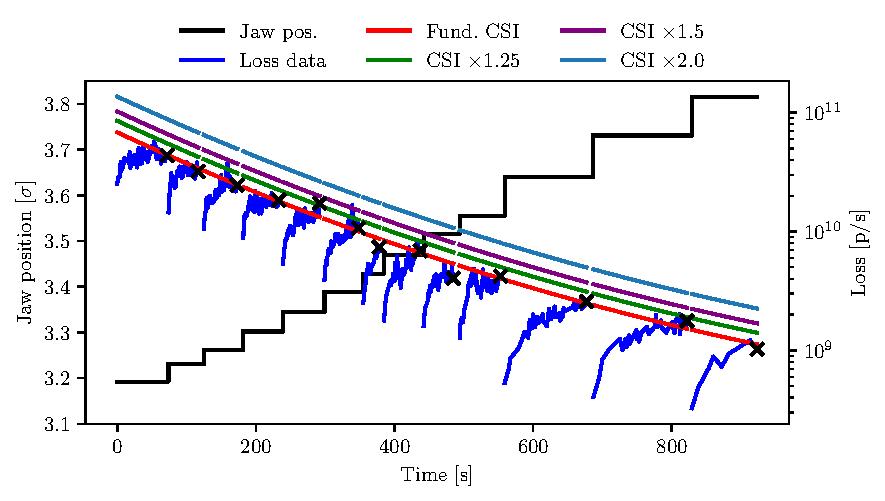
\includegraphics[trim={0 2.5mm 0 3mm}, clip, width=\columnwidth]{5_Diffusion_measurement_LHC/figs/second_bis.pdf}
    \caption{Estimates of $J_\mathrm{eq}(t)$ for Beam~1 data. An initial estimate is made with a CSI with positive second derivative passing through the end points of the measured recovery currents. The various curves are obtained by multiplying the fundamental CSI by a constant term, and represent estimates of the partial recovery currents.}
    \label{fig:second}
\end{figure}
%

To cope with the rapid sequence of jaw movements, we replace the integral terms in Eq.~\eqref{eq:difference} with the approximation
\begin{equation}
    \rho_{\mathrm{app}}^{*}(I)= \begin{cases} -M & \text { if } I\leq I_{\mathrm{a}}\\ -\left(\frac{I_{\mathrm{a}}^{\prime }-I}{I_{\mathrm{a}}^{ \prime}-I_{\mathrm{a}}}\right) M & \text { if } I>I_{\mathrm{a}} \, , \end{cases} 
\end{equation}
where $M$ is a constant fixed for each jaw movement that represents an unknown amount of out-of-equilibrium distribution.
A scan is performed on different combinations of CSI and $M$ values while keeping track of $\chi^2$ achieved by the fitting routine that determines the values of the model parameters $\kappa, I_\ast$. The result of this procedure is shown in Figs.~\ref{fig:fourth} and~\ref{fig:fifth}, where one can observe the existence of an optimal configuration of parameters and the good reconstruction performance achieved by such a configuration. The optimal fit results for Beam~1 and Beam~2 data are reported in Table~\ref{tab:fit_results}.

\begin{figure}
    \centering
    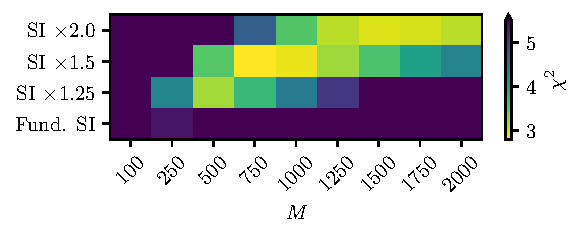
\includegraphics[trim={0 2.5mm 0 1.5mm}, clip, width=0.98\columnwidth]{5_Diffusion_measurement_LHC/figs/fourth.pdf}
    \caption{Fit performance for Beam~1 data vs. CSI and $M$ values, showing the existence of an optimal configuration.}
    \label{fig:fourth}
\end{figure}
%
\begin{table}[htb]
    \centering
    \caption{Results of the fit procedure, along with corresponding setup for CSI and $M$ values.}
    \begin{tabular}{lcccc}
        \toprule
        Beam / Plane & CSI & $M$ & $\kappa$ & $I_\ast\ [\sigma]$ \\
        \midrule
        Beam~1 / V & $\times1.5$ & $750$ & $0.59\pm0.03$ & $21\pm2$ \\
        Beam~2 / V & $\times1.5$ & $1000$ & $0.85\pm0.02$ & $39\pm8$ \\
        \bottomrule
    \end{tabular}
    \label{tab:fit_results}
\end{table}
%

Note that the values reported in~\cite{bazzani2020diffusion}, namely $\kappa=0.33 $ and $I_\ast \simeq 21$, were obtained for Beam~2 and considering the diffusion in the vertical plane. It should be stressed that these previous measurements were performed with isolated bunches, whereas in the beam measurements analysed here, beam-beam effects were present. 

\begin{figure}[htb]
    \centering
    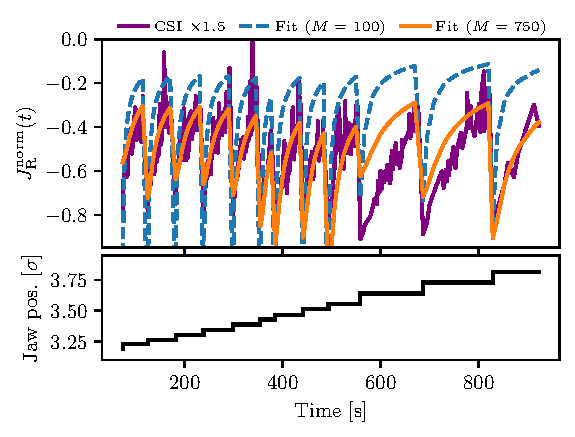
\includegraphics[trim={0 2.5mm 0 3mm}, clip, width=0.95\columnwidth]{5_Diffusion_measurement_LHC/figs/fifth.pdf}
    \caption{Fit results for Beam~1 data for two $M$ values. The optimal value (orange) outperforms a lower value (blue).}
    \label{fig:fifth}
\end{figure}
%
\section{Conclusions and outlook}
%
A non-linear diffusive model based on Nekhoroshev theorem was used to reconstruct available beam loss data obtained at the  LHC from collimator scans. The differences between the approach used to gather the data and the optimal one suggested by our recent numerical studies required adaptation of some of the key elements of our fitting procedure. Eventually, this led to good reconstruction performances and promising insights into the global diffusive behaviour of the LHC beam halo.

Future research will focus on acquiring beam data using the proposed optimised experimental method to characterise more accurately the presence of nonlinear diffusive behaviour. The new datasets might also be used to perform comparisons between the newly proposed collimator scan method for the Nekhoroshev-based diffusive model and the previous approach based on the linearisation of the diffusion coefficient around a given jaw position.

\section{Application of the measurement protocol}

\subsection{Experimental results}

